\documentclass[10pt]{beamer}
\usepackage[utf8]{inputenc}
\usepackage{xeCJK}
\usepackage{graphicx}
\usepackage{mathtools}
\usepackage{utopia} %font utopia imported
\usepackage{geometry}
\usetheme{CambridgeUS}
\usecolortheme{dolphin}


% set colors
\definecolor{hkustyellow}{RGB}{167, 131, 55}
\definecolor{hkustblue}{RGB}{0, 56, 116}
\definecolor{hkustred}{RGB}{209, 51, 59}
\setbeamercolor*{palette primary}{bg=hkustblue, fg = white}
\setbeamercolor*{palette secondary}{bg=hkustred, fg = white}
\setbeamercolor*{palette tertiary}{bg=hkustyellow, fg = white}
\setbeamercolor*{titlelike}{fg=hkustblue}
\setbeamercolor*{title}{bg=hkustblue, fg = white}
\setbeamercolor*{item}{fg=hkustblue}
\setbeamercolor*{caption name}{fg=hkustblue}
\usefonttheme{professionalfonts}
\usepackage{natbib}
\usepackage{hyperref}
%------------------------------------------------------------
\titlegraphic{
\includegraphics[height=2.5cm]{logoUA.png}}
% \usepackage{fontspec}
% \setmainfont{Times New Roman}


\setbeamerfont{title}{size=\large}
\setbeamerfont{subtitle}{size=\small}
\setbeamerfont{author}{size=\small}
\setbeamerfont{date}{size=\small}
\setbeamerfont{institute}{size=\small}
\setbeamertemplate{background}{%
    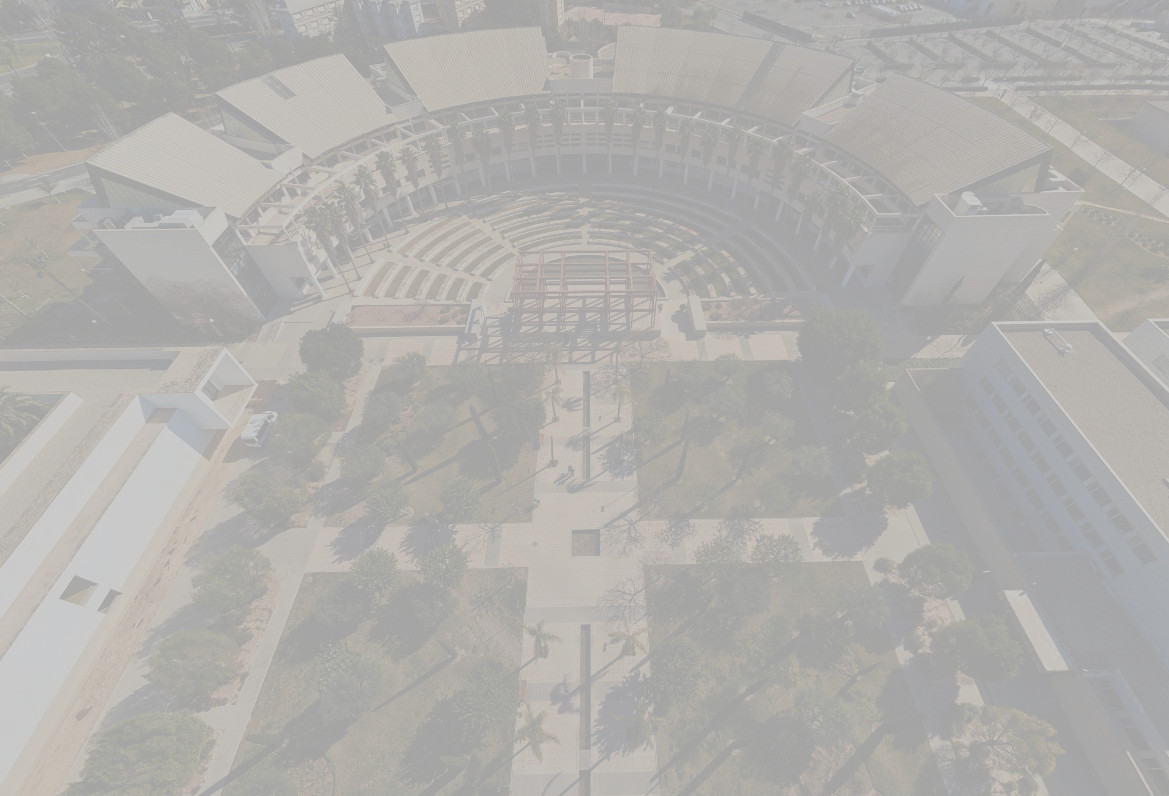
\includegraphics[width=\paperwidth,height=\paperheight]{aulario 2.jpg}
}

\title[Universidad de Alicante]{\textrm{\textbf{Práctica Demostrativa}}}
\subtitle{\textrm{Termomagnetismo}}
\author[vmr48@alu.ua.es y amhm10@alu.ua.es]{\textrm{Víctor Mira Ramírez y Ahlam Makboul Hilal}}

\institute[]{\textrm{Universidad de Alicante}}
\date[\today]{\textrm{\today}}

%------------------------------------------------------------
%This block of commands puts the table of contents at the 
%beginning of each section and highlights the current section:
%\AtBeginSection[]
%{
%  \begin{frame}
%    \frametitle{Contents}
%    \tableofcontents[currentsection]
%  \end{frame}
%}
\AtBeginSection[]{
  \begin{frame}
  \vfill
  \centering
  \begin{beamercolorbox}[sep=8pt,center,shadow=true,rounded=true]{title}
    \usebeamerfont{title}\insertsectionhead\par%
  \end{beamercolorbox}
  \vfill
  \end{frame}
}
%------------------------------------------------------------

\begin{document}

%The next statement creates the title page.
\frame{\titlepage}
\begin{frame}
\frametitle{\textrm{Índice}}
\tableofcontents
\end{frame}
%------------------------------------------------------------
\section{\textrm{Introducción}}
    \subsection{Descripción del experimento}
    \begin{frame}{\textrm{Descripción del experimento}}

    \end{frame}
    \subsection{Contexto histórico}
    \begin{frame}{\textrm{Contexto histórico}}

    \end{frame}

%------------------------------------------------------------
\section{\textrm{Hipótesis Inicial}}
    \begin{frame}{\textrm{Hipótesis Inicial}}

    \begin{block}{Hipótesis}

    Hechos observables: El clip se calienta, y cae. 
    Relación calor/magnetismo. 
    
    Al calentar el clip, este pierde sus propiedades ferromagnéticas, y deja de ser atraído por el imán. 
    \end{block}


    \end{frame}
%---------------------MARCO TEORICO-----------------------------
\section{\textrm{Marco Teórico}}
    \subsection{\textrm{Materiales Paramagnéticos y Ferromagnéticos}}
        \begin{frame}{\textrm{Materiales Paramagnéticos y Ferromagnéticos}}
            \begin{block}{Paramagnetismo}
                El paramagnetismo es el fenómeno que se da en el momento que las moléculas que se encuentran en una sustancia tiene un magnetismo estable. De la misma manera, aparece cuando los materiales se magnetizan cuando están en contacto con un campo magnético externo. Este fenómeno aparece cuando algunos electrones no están emparejados.
            \end{block}
        \end{frame}
        \begin{frame}{\textrm{Materiales Paramagnéticos y Ferromagnéticos}}
            \begin{block}{Ferromagnetismo}
                El ferromagnetismo es una propiedad que poseen algunos materiales en los cuales los espines de los electrones que se conoce como dominio magnético se colocan paralelamente. En este caso la temperatura le afecta directamente ya que puede alterar el desorden si la temperatura se va incrementando, todos los materiales ferromagnéticos tienen una temperatura característica que se conoce como temperatura Curie $T_c$.
            \end{block}
        \end{frame}



        
    \subsection{\textrm{Temperatura de Curie}}
    \begin{frame}{\textrm{Temperatura de Curie}} 
        \begin{block} {Desmagnetización}

        Ferromagnetismo  $\rightarrow$   Paramagnetismo

        \end{block}

        
        \begin{block} {Ley de Curie - Susceptibilidad magnética}


            \begin{columns}
            \column{0.5\textwidth}
                        \begin{equation*} 
                        X_m=\frac{C}{T}
                        \end{equation*}
            \column{0.5\textwidth}
            Capacidad de un material para magnetizarse
            \end{columns}
       
        \end{block}
        
       
    \end{frame}

%---------------------------- APLICACION--------------------
\section{\textrm{Aplicación}}
    \subsection{\textrm{Motor de Tesla}}
        \begin{frame}{\textrm{Motor de Tesla}}

        \end{frame}
    \subsection{\textrm{Funcionamiento}}
        \begin{frame}{Funcionamiento}
            \begin{block}{Ciclo del Motor}
                    \newline Objeto atraído por el imán.
                    \newline Se calienta hasta la Tª Curie.
                    \newline Pierde sus propiedades ferromagnéticas.
                    \newline Se aleja del imán.
                    \newline Se enfría. 
            \end{block}
            
            \begin{figure}
                \centering
                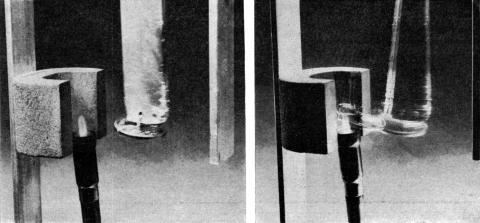
\includegraphics[scale=0.4]{image.png}
                \caption{Prototipo de Tesla}
                \label{fig:Tesla}
            \end{figure}
        \end{frame}

    \begin{frame}{Ejemplo visual}

    % \begin{figure}
    %     \centering
    %     \includegraphics{ezgif.com-video-to-gif.gif}
    %     \caption{Ejemplo de un motor termomagnético }
    %     \label{fig:gif}
    % \end{figure}
        
    \end{frame}

%------------------------------------------------------------
\end{document}
